

\chapter{Хранение и передача данных}


\section{RS-триггер}

Триггер --- это простейшее устройство для хранения одного бита информации.
Если он включен, там хранится единица, а если выключен --- хранится ноль.

Хранение одного бита можно сделать с помощью одного реле.
Если оно включается, то сохранена единица.
Чтобы это включённое состояние запоминалось, нужно организовать обратную
связь через один из контактов. Как только реле включается с помощью
входа $SET$, на его
обмотку подаётся напряжение через его же замкнутый контакт. Поэтому даже
если перестать подавать напряжение на вход $SET$, реле всё равно останется включённым:

\begin{center}
\includegraphics{schemes/trigger1.png}
\end{center}

Но если такое реле уже включилось, выключить его не получится. Единственный способ ---
это снять питание. Тогда контакты разомкнутся и при повторной подаче питания реле будет
в выключенном состоянии.

Чтобы не отключать всю схему, нужно предусмотреть отдельное реле, позволяющее
отключить питание только для этой схемы:

\begin{center}
\includegraphics{schemes/trigger2.png}
\end{center}

Теперь подав сигнал на вход $RESET$ можно сбросить триггер. И там опять окажется ноль.

Триггер с двумя входами $RESET$ и $SET$ называется RS-триггером.
На практике удобно объединить несколько таких триггеров в многобитовый регистр
и использовать для них единый сигнал сброса, сэкономив несколько реле.

\section{Шина}

Шина --- это набор проводников, объединённых общим назначением.
К этим проводникам подключаются несколько устройств для обмена сигналами.

Например, по шине данных процессор может читать или записывать данные из памяти
или жёсткого диска. Шина адреса используется для выбора определённой ячейки в памяти.
А по шине управления приходят сигналы, позволяющие отличать обращение к памяти
от обращения к диску.

Так как к шине обычно подключается больше одного входа и больше одного выхода,
необходимо изолировать лишние устройства, когда шина используется другими.
В релейном компьютере мы можем использовать для подключения к четырёхбитной шине
шинный формирователь из одного реле:

\begin{center}
\includegraphics{schemes/bus.png}
\end{center}

Когда такое реле включается, оно может соединить какое-то устройство (например, регистр)
с шиной. Подключение будет двунаправленным, поэтому с помощью этой схемы можно как
записывать данные в регистр, так и считывать оттуда.

Шинные формирователи подключаются к каждому устройству, поэтому
для передачи данных и вычислений требуется формировать множество сигналов $SELECT$.

\section{Шины в конструкторе}

В конструкторе все компоненты соединяются с помощью восьмибитных шлейфов.
В каждом из них есть питание и земля. Кроме того, большинство из таких
подключений это шина в которой от $1$ до $4$ сигналов.

Например, $4$ сигнала могут использоваться для управления модулем регистра.
Или для передачи данных из одного регистра в другой.
Каждым из таких сигналов можно управлять с помощью модуля переключателей,
соединив его с соответствующей шиной.

\section{Регистр}

Регистры внутри процессоров (или периферийных устройств)
используются для хранения данных и для проведения вычислений.
Регистры могут иметь выделенное назначение (например, хранить режим работы устройства)
или же используются почти для всего (адрес, операнд арифметических операций,
значение для ввода-вывода).

\begin{center}
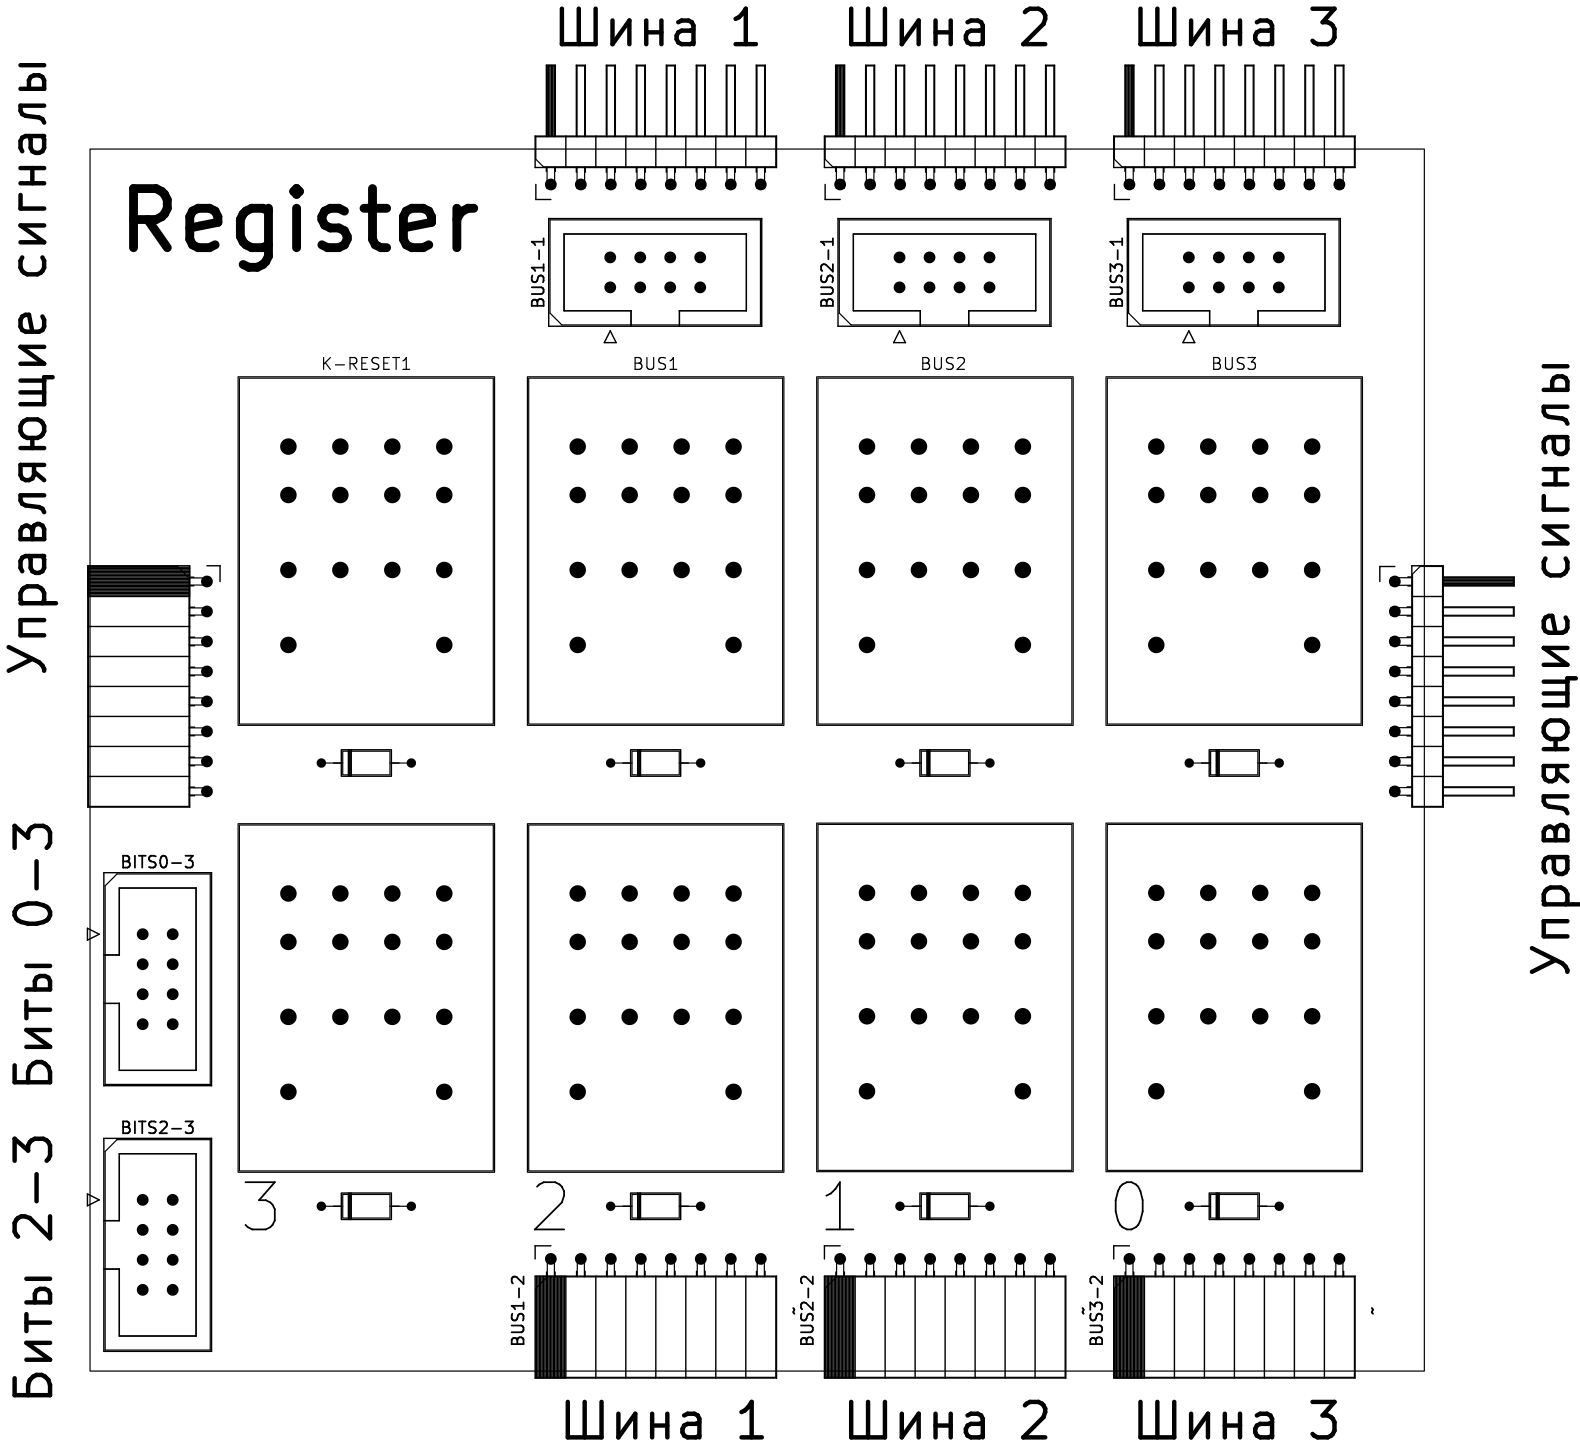
\includegraphics{boards/register.png}
\end{center}

Модуль четырёхбитного регистра состоит из четырёх реле-триггеров,
одного реле для обнуления регистра и трёх реле для подключения
к шинам данных.

Для хранения данных используются RS-триггеры, описанные выше,
но сигнал для сброса у них общий. Таким образом, записывать
данные можно только во все четыре бита сразу. Поэтому такой
модуль и реализует функции цельного регистра, а не нескольких
разрозненных RS-триггеров.

Также модуль регистра содержит три шинных формирователя.
Их можно использовать для подключения триггеров к разным устройствам
через три шины. Например, одна шина может быть предназначена
для первого операнда при вычислениях, вторая для второго операнда,
а третья для копирования данных между регистрами.

Если в модуль установить только реле шинных формирователей,
получится модуль, который может подключать четырёхбитные сигналы
(полученные из разъёма для прямого чтения значений триггеров) к одной
из выбранных шин.

Модуль регистра имеет следующие разъёмы:
\begin{itemize}
  \item Слева и справа: управляющие сигналы сброса и выборки.
        Можно подключить тумблеры
        для ручного включения сигналов. Также можно соединить несколько
        модулей регистра, чтобы управлять одним набором сигналов сразу
        для $8$, $12$ \ldots бит.
  \item Сверху и снизу: три шины данных. Реле регистра могут
        подключаться к шинам для записи или чтения данных.
  \item Дополнительные разъёмы с битами $0-3$ и $2-3$ для чтения или
        записи значения без подключения к шине.
\end{itemize}

Чтобы прочитать значение регистра нужно активировать сигнал выборки
его на нужную шину. А уже через шину сигналы поступят на вход какой-то
другой схемы.

Для записи значения в регистр нужно сначала обнулить его триггеры,
иначе запись не произойдёт в тех битах, где уже хранятся единицы.
После этого регистр подключается к нужной шине, и триггеры
защёлкивают нужное значение.

\subsection{Практикум}

Протестировать работу регистра можно собрав следующую схему:

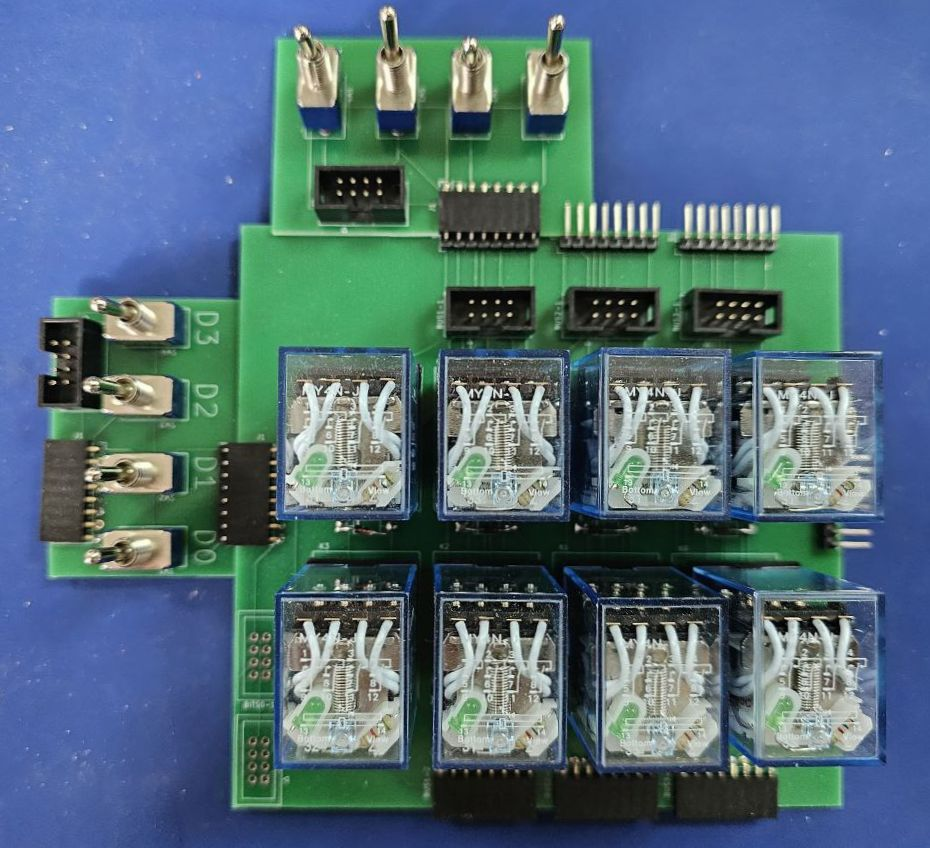
\includegraphics[width=0.5\columnwidth]{photo/register.jpg}

\begin{itemize}
  \item Тумблеры слева управляют работой регистра. Бит 0 --- обнуление, бит 1 --- выборка на шину 1.
  \item Тумблеры сверху нужны для ввода значения регистра. Когда он подключается к шине 1,
        значения, набранное на тумблерах, записывается в регистр.
\end{itemize}

\subsubsection{Регистр без шины}

\begin{enumerate}
    \item Подключить тумблеры проводом к битам $0-3$ вместо шины.
    \item Набирать значение, убедиться, что биты переключаются в $1$, но не возвращаются в $0$.
    \item Обнулить тумблеры с данными.
    \item Включить и выключить сигнал сброса. Убедиться, что значения всех битов теперь $0$.
\end{enumerate}

\subsubsection{Регистр с шиной}

\begin{enumerate}
    \item Отключить все управляющие сигналы.
    \item Набрать значение на тумблерах для данных. Убедиться, что это не влияет на регистр.
    \item Включить и выключить сигнал выборки на шину $1$. Убедиться, что данные записались в регистр.
    \item Включить и выключить сигнал сброса. Убедиться, что значения всех битов теперь $0$.
\end{enumerate}

\subsection{Задачи}

\begin{enumerate}
    \item Придумайте, как скопировать данные из одного регистра в другой, не запоминая их в голове.
\end{enumerate}


\section{Шина и регистровый файл}

Несколько регистров можно соединить в регистровый файл.
Регистровый файл --- это набор регистров. Он может быть однородным
(все регистры эквивалентны) или нет (разные регистры имеют разное назначение).

У каждого из регистров есть сигналы выборки на одну из трёх шин.
Если два регистра подключены к одной шине одновременно,
то значения одного будут копироваться в другой. Если точнее,
включённые биты включают аналогичные в другом регистре, то есть
копирование возможно в обе стороны одновременно.

Нулевые биты при этом копироваться не могут. Для записи нулей
регистр необходимо сбросить.


\subsection{Практикум}


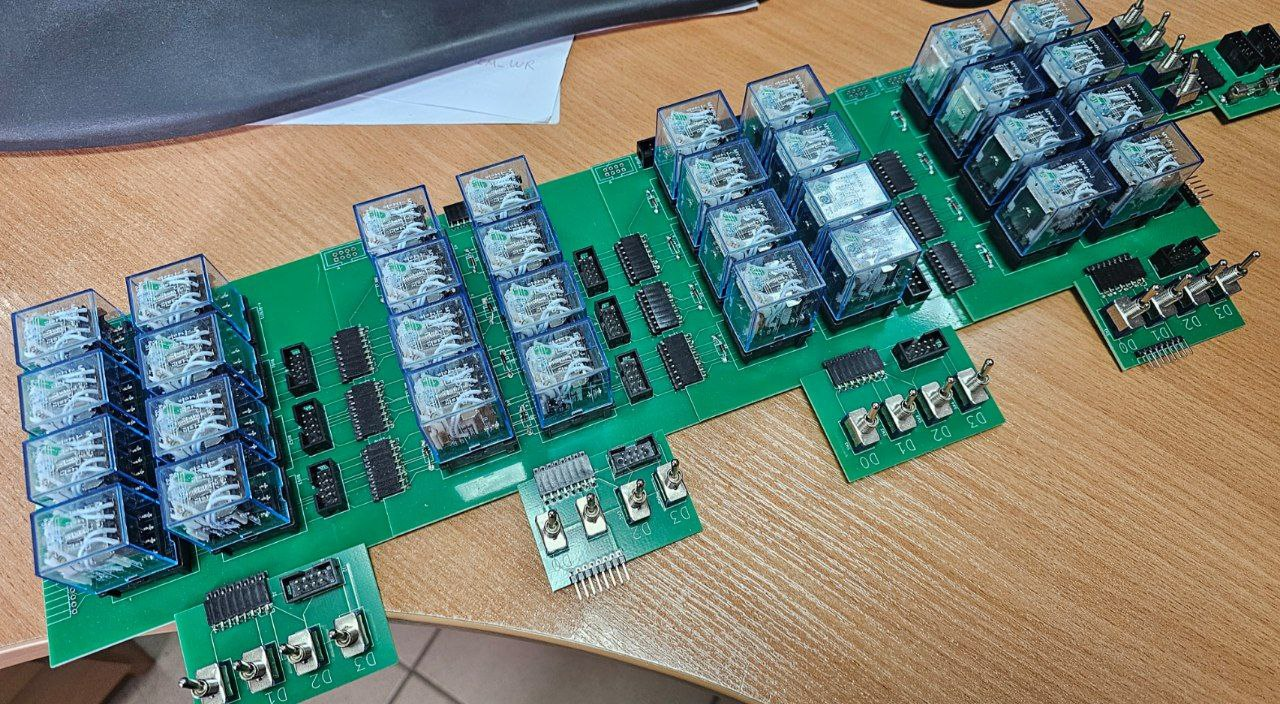
\includegraphics[width=\columnwidth]{photo/register_file.jpg}

Запись в регистры:

\begin{enumerate}
    \item Отключить все управляющие сигналы.
    \item Набрать значение на тумблерах, подключённых к шине данных $1$.
    \item Подключить с помощью тумблера регистр к шине $1$. Убедиться, что в него записалось набранное значение.
    \item Отключить регистр от шины.
    \item Подключить другой регистр к шине $1$. Убедиться, что в него записалось набранное значение.
\end{enumerate}

Копирование значения:

\begin{enumerate}
    \item Отключить все управляющие сигналы.
    \item Подключить регистр с ненулевыми битами к шине $2$.
    \item Подключить пустой регистр к шине $2$. убедиться, что он получил такое же значение, что и в первом регистре.
    \item Отключить все управляющие сигналы.
    \item Аналогично проверить шину $3$.
\end{enumerate}

